\documentclass[oneside,b5paper,11pt]{book} %book class in 11 points
\usepackage{geometry} % Package re-sizing page for b5paper
\usepackage[hangul]{kotex} % Korean support
\usepackage{natbib} % cite style
\usepackage{paralist} % package for inline enumerate, i) ii)...

\usepackage{graphicx} % Allows including images

\usepackage{amsmath} % for math symbols
\usepackage{amssymb} % for math symbols

\usepackage{tablefootnote} % to use table foot note

%\graphicspath{ {D:/_PlayGround/Github/2016_thesis/tex/images} }
\graphicspath{ {C:/My/Playground/Git/2016_Thesis/tex/images/} }

\kscntformat{section}{}{} % 제 1.1절 -> 1.1
\renewcommand\thesection{\arabic{section}.} % 제 1.1절 -> 1.1
\renewcommand\thesubsection{\indent\arabic{section}.\arabic{subsection}.}


%%들여쓰기
\usepackage{indentfirst}
\setlength\parindent{2.0em}




\title{석사 학위 논문 초안}
\author{김동완}
\date{\today}

\begin{document}

\maketitle

\tableofcontents

\chapter{서론}

\section{개요}
최적화(optimization) 알고리즘의 하나인 경사하강법(Gradient descent)에서는 전체 샘플 데이터를 스캔 할 때마다 회귀 계수 추정치를 갱신해 나간다. 비용함수(cost function)를 $J(w) = \frac{1}{2} \sum_{i}(target^{(i)} - output^{(i)})^{2}$ 라 할때 길이가 j인 계수 벡터(weight vector) $w_i$를 $w_{i+1}=w_{i}+\Delta w$로 갱신하는 매 반복에서 $j$개의 모수 추정치($w$)를 얼마만큼 줄일지 혹은 늘릴지 $\Delta w$ 값을 결정해야 한다. 여기에서 $\Delta w$는 아래와 같다.
\begin{eqnarray}
\Delta w_{j} 	&=& -\alpha \frac{\delta J}{\delta w_{j}} \\
							&=& -\alpha \sum_{i}(target^{(i)} - output^{(i)})(-x^{(i)_{j}}) \\
							&=& \alpha \sum_{i}(target^{(i)} - output^{(i)})(x^{(i)_{j}})
\end{eqnarray}
즉 비용함수(cost function)의 경사도가 크면 그만큼 많이 $w$값을 수정하게 되는데, 학습 계수(learning rate, step size) $\alpha$에 비례하여 수정치가 결정된다.

 경사하강법에서는 한번 $w$값을 수정하기 위하여 전체 샘플 데이터를 스캔하게 된다. 그런데 이런 방식은 샘플의 수가 많은 경우 
비용함수 $J(w)$를 최소로 하는 $w$값을 찾기 까지 그 처리 시간이 길어 지게 된다. 모수에 대한 학습(learning)이나 추론(inference)를 진행할 때 데이터의 크기가 작거나 데이터의 수집으로부터 예측까지 시간적 여유가 있을 경우 데이터 전체를 한꺼번에 활용하는 일괄 처리(batch processing) 방식을 사용한다. 반면 데이터를 한꺼번에 처리하기에 그 크기가 지나치게 크거나 스트리밍(streaming)으로 유입되는 데이터에 대해서 실시간으로 예측을 처리해야 하는 경우 온라인 학습(online learning)을 사용해야 할 필요성이 있다.

 이처럼 매 갱신에서 전체 샘플 데이터를 사용하는 대신 샘플 하나 혹은 일부분만을 사용하여 $w$ 값을 갱신해 가는 경사하강법을 확률적 경사 하강법(Stochastic Gradient Descent, Online Gradient Descent)이라 하며, 확률적 이라는 단어에서 알 수 있듯이 $J(w)$를 최소로 하는 $w$값을 확률적 근사방법으로 찾아가는 것이다. 하나의 샘플만을 이용해 $w$의 갱신 방향과 크기를 결정하기 때문에 경사하강법과는 달리 $J(w)$값이 커지는 경우도 있으나 샘플 수가 충분할 경우 $J(w)$의 전역 최소값으로 수렴하는 $w$를 찾을 수 있는 것으로 알려져 있다. \citep{Bottou2010}

 경사 하강법 혹은 확률적 경사 하강법의 성능을 결정하는 가장 중요한 요소는 학습 계수(learning rate) $\alpha$인데, 모형이 근사적으로 수렴하기 위해서는 이 값을 점차 줄여나가야만 한다. $\alpha$ 값을 줄여 나가는 방법으로는 반복(iteration)의 진행횟수에 비례하여 $\alpha_{t+1} = \alpha_{t} / (1 + t \times d )$와 같이 $\alpha$ 값을 감소 시키는 방법이나, 알고리즘의 성능에 따라 $\alpha$값을 변화시키는 방법 등이 있다. 

 회귀 모형과 같이 선형 가우시안을 가정하는 경우 이 문제를 \citet{Kalman1960}의 칼만 필터(Kalman filter)와 같이 접근할 수도 있다. 온라인 학습에서 가장 가까운 미래 시점의 모수 값 혹은 분포를 추정하는 것을 흔히 필터링(filtering)이라 하고, 과거 시점의 그것을 추정하는 것을 스무딩(smoothing)이라 한다. 온라인 필터링 알고리즘으로는 칼만 필터\citep{Kalman1960}, 칼만 필터의 비선형 버전이라 할 수 있는 확장 칼만 필터\citep{Smith1962}, 무향 변환(unscented transform)을 이용한 가우시안 근사로 확장 칼만 필터를 개선한 무향 칼만 필터\citep{Julier1997}, 사전 분포와 측정값을 이용하여 적률 대응(moment matching)으로 사후 분포를 근사하는 추정된 밀도 필터(Assumed Density Filtering)\citep{Opper1996} 등이 있다.
 
 추정된 밀도 필터(Assumed Density Filtering)은 베이지안 접근 방법으로서 \citet{Opper1996}가 제안한바 있는데, 매 반복마다 하나의 샘플을 이용하여 $w$값을 갱신하는데 있어서 $t$ 시점에서 $w$의 분포를 생각하고 이때 사용할 하나의 샘플을 이용하여 사후 분포를 구한다. 다시 $t+1$ 시점에서는 이전 시점에서의 사후 분포를 사전분포로 활용하여 계속하여 $w$의 분포를 갱신해 나가는 것이다. 이러한 접근 방법은 $w$의 위치와 불확실성을 해당 분포의 평균과 분산으로 모형화한 것이라 할 수 있다. 

 본 논문에서는 이러한 기존의 연구결과들(\citet{Bottou2010}; \citet{Opper1996}을 샘플 수가 수천만건에 이르고 다수의 범주형 변수, 그리고 범주의 개수가 유동적인 대규모 데이터에 적용하기 위한 방법을 고려해 보고 각 방법의 특성에 대해서 고찰해 볼 것이다. 또한 가상 데이터와 실제 데이터에에 각 방법론의 적용해 보고 각각의 특성을 실증적으로 살펴볼 것이다. 이를 위해 먼저 3장 1절 에서는 가상 데이터를 생성하여 SGD와 ADF 방법을 적용해 볼 것이다. 그리고 3장 2절에서 소규모 이항반응 데이터에 두 방법을 적용해 볼 것이며 3장 3절에서는 사례연구(대규모 이방반응 데이터)를 통해서 SGD와 ADF에 대한 실증적 비교 분석을 실시한다. 마지막으로 4장에서는 본 논문의 결론과 향구 과제를 논의한다.

 
%
% Chapter 1
%정
\chapter{가우시안 구적법을 이용한 온라인 베이지안 로지스틱 회귀 모형}
 
% Section 1-
\section{로지스틱 회귀 모형}

일반화 선형 모형은 크게 
\begin{inparaenum}[i)]
\item 반응변수 $Y$와 그것의 확률 분포,\quad
\item 설명변수와 회귀계수의 선형식(systematic component), $\eta = \theta^T x$, \quad
\item 연결함수(link function), $g(\cdot)$ 로 구성된다.
\end{inparaenum} 이 3가지 구성요소는 아래와 같이 '반응변수 $Y$의 기댓값 $\mu$와 선형식 $\eta$의 관계가 연결함수로 표현되는 형태로 결합된다.\citep{Agresti1996}
$$E(Y) = \mu = g^{-1}(\theta^T x)$$

 로지스틱 회귀 모형은 일반화 선형 모형의 한 가지 형태로서 반응변수 $Y$가 이항분포를 따르고 연결함수가 
$$
g(\mu) = logit(\mu) =log \left(\frac{\mu}{1-\mu}\right)
$$
위와 같은 log-odds(logit)인 경우를 말한다.

결국 반응변수 $Y$는 성공확률 $\pi$가 $g^{-1}(\theta^T x)$인 이항분포로서, 아래와 같이 $\pi$를 회귀계수 혹은 가중치(weight)와 설명변수의 선형결합을 인자로 하는 로지스틱(logistic, sigmoid) 함수로 표현할 수 있다.
$$
\pi_i = P(y_i=1) = \frac{1}{1+exp(-\theta_i^T x_i)}
$$

\begin{eqnarray}
    {}logit(E[Y])  
  &=& logit(P(Y=1))  \\
  &=& logit(\pi(x))  \\  
  &=& log \left( \frac{\pi(x)}{1-\pi(x)}\right) \\
  &=& \theta^T x
\end{eqnarray}


% Section 1-
\section{추정된 밀도 필터링(Assumed-density filtering)}
 추정된 밀도 필터링(Assumed-density filtering, ADF)는 베이지안 네트워크 혹은 여타의 통계 모형에서 사후분포를 근사적으로 계산하는 방법으로서 통계학에는 \citet{Lauritzen1992}에서 제안된 바 있다. 또한 분야에 따라 "추정된 밀도 필터링(Assumed-density filtering)", "온라인 베이지안 학습(On-line Bayesian learning)", "적률 대응(Moment matching)", "약한 주변화(Weak marginalization)"이라 부르기도 한다. \citep{Minka2013}

 ADF에서는 사후분포를 가우시안과 같은 특정 분포로 근사하는 방법으로서 예측-갱신-투영(predict-update-project)과정을 반복한다. 예측(predict) 과정에서는 모수 $\theta$에 대한 $t-1$ 시점의 사전분포, $q_{t-1}(\theta_{t-1})$와 $t$시점의 관측치를 이용하여 이후 시점 $t$에서의 $\theta$에 대한 사후예측분포, $q_{t|t-1}(\theta_{t})$를 구하고, 갱신(update) 과정에서는 앞서 구한 사전분포와 사후예측분포를 이용하여 $\theta$에 대한 사후분포, $\hat{p}(\theta_t)$를 구한다. 마지막으로 이 사후 분포가 다루기 쉬운 형태가 아닌 경우가 빈번하기 때문에 다루기 쉬운 분포로 투영(project)하는 과정을 거치게 된다.

\begin{itemize}
\item 근사 사전분포: 
$$q_{t-1}(\theta_{t-1}) \approx p(\theta_{t-1}|y_{1:t-1})$$
\item 1단계 사후예측분포: 
$$q_{t|t-1}(\theta_t) = \int p(\theta_t | \theta_{t-1}) q_{t-1}(\theta_{t-1}) d\theta_{t-1}$$
\item 사후분포:
$$\hat{p}(\theta_t) = \frac{1}{Z_t}p(y_t | \theta_t)q_{t|t-1}(\theta_t)$$
\item 정규화 상수(normalizing constant):
$$Z_t = \int p(y_t | \theta_{t-1})q_{t|t-1}(\theta_{t})d\theta_{t}$$
\item 근사 사후분포:
$$q(\theta_t) = \arg\min_{q \in Q} \mathrm{KL}(\hat{p}(\theta_t || q(\theta_t)) $$
\end{itemize}

근사 사후분포를 구할 때 위와 같이 쿨백-라이블러 발산값(Kullback-Leibler divergence)을 최소화하는 함수 $q(\theta_t)$를 구하는데 이는 (다루기 어려운)사후분포$\hat{p}(\theta_t)$를 다루기 쉬운 분포 공간으로 투영(project)하는 것이라 생각할 수 있다. 그런데 투영하려는 분포 $q$가 지수족에 속할 경우 단순히 적률 대응(moment matching)만으로 $q(\theta_t)$를 구할수 있다.\citep{Murphy2012}


% Section 1-
\section{일반화 선형 모형에서의 가우시안 근사}
편의를 위해 설명변수와 회귀계수의 선형식(systematic component)을 $s_t=\theta_t^T x_t$라 하자. 만약 $\theta_t$에 대한 1단계 사후예측분포, $q_{t|t-1}(\theta_t)$가 \newline 
$\prod_i N(\theta_{t,i};\mu_{t|t-1,i},\sigma^2_{t|t-1,i})$라면 $s_t$의 사후 예측분포, $q_{t|t-1}(s_t)$ 는 아래와 같다.
\begin{eqnarray}
   q_{t|t-1}(s_{t}) &\equiv& N(s_t;m_{t|t-1}, {v}_{t|t-1})
\\ m_{t|t-1} &=& \sum^N_{i=1}x_{t,i}\mu_{t|t-1,i}
\\ {v}_{t|t-1} &=& \sum^N_{i=1}x^2_{t,i}{\sigma}^2_{t|t-1,i}
\end{eqnarray}

이때 $s_t$의 사후분포, $q_t(s_t)$는 아래와 같다.
\begin{eqnarray}
q_t(s_t) &\equiv& N(s_t; m_t, v_t)
\\ m_t &=& \int s_t \frac{1}{z_t} f(y_t|s_t) q_{t|t-1}(s_t)ds_t \label{eq:10}
\\ v_t &=& \int s^2_t \frac{1}{z_t} f(y_t|s_t) q_{t|t-1}(s_t) ds_t - m_t^2 \label{eq:11}
\\ z_t &=& \int f(y_t|s_t) q_{t|t-1}(s_t)ds_t \label{eq:12}
\\ f(y_t|s_t) &\equiv& Ber(y_t;\pi = sigmoid(s_t))
\\ & =& \pi^{y_t} (1-\pi)^{(1-y_t)}, \quad y_t \in \{0,1\}
\\ & =& \left(\frac{1}{1+exp(-s_t)}\right)^{y_t} \left(\frac{exp(-s_t)}{1+exp(-s_t)}\right)^{(1-y_t)}, \quad y_t \in \{0,1\} \nonumber
\end{eqnarray}

위의 적분식을 계산하기 위하여 가우시안 구적법(Gaussian quadrature)을 사용할 수 있다. 가우시안 구적법을 이용하면 어떤 다항식과 알려진 함수 $W(x)$의 곱에 대한 계산을 아래와 같이 다항식 함수값의 가중합으로 근사할 수 있다.
$$\int^b_a W(x)f(x)dx \approx \sum^N_{j=1}w_j f(x_j)$$
특히 $W(x)=e^{-x^2}$와 어떤 함수의 곱을 적분하는 경우, $\int^{+\infty}_{-\infty}e^{-x^2}f(x)dx$, 가우스-에르미트 구적법(Gauss-Hermite quadrature)을 사용할 수 있다. $\chi'$를 결정점(sample point)이라 하고 $\omega'$를 가중치(weight)라고 할때,  $\chi=\chi'\sqrt{2}\sigma_{s_t}+\mu_{s_t}$와 $\omega_i = \frac{\omega'}{\sqrt{\pi}}$로 변수변환할 수 있다. 이를 이용하여 앞서 \ref{eq:10}, \ref{eq:11}, \ref{eq:12}의 적분을 아래와 같이 근사할 수 있다.\citep{Zoeter2007}

\begin{eqnarray}
q_t(s_t) &=& N(s_t; \tilde{m}_t, \tilde{v}_t)
\\ \tilde{m}_t &=& \frac{1}{\tilde{z}_t} \sum_i \chi_i f(y_t; \chi_i ) \omega_i
\\ \tilde{v}_t &=& \frac{1}{\tilde{z}_t} \sum_i \chi^2_i f(y_t; \chi_i ) \omega_i - \tilde{m}^2_t
\\ \tilde{z}_t &=& \sum_i f(y_t; \chi_i ) \omega_i
\end{eqnarray}

이렇게 구한 $s_t$의 사후분포를 이용하여 $\theta$의 근사 사후분포,  $q(\theta_t)$를 구할 수 있다. $q_{t|t-1}(s_{t-1})$을 $q_{t}(s_t)$로 갱신한 후 평균과 분산의 변화를 각각 $\sigma_m = m_t - m_{t|t-1}$과 $\sigma_v = v_t - v_{t|t-1}$라고 하면, $t$시점의 $i$번째 $\theta$의 분포는 아래와 같다.\citep{Murphy2012}
\begin{eqnarray}
   q(\theta_t,i) &\sim& N(\theta_{t,i};\mu_{t,i}, \sigma^2_{t,i})
\\ \mu_{t,i} &=& \mu_{t|t-1,i} + a_i \delta_m
\\ \sigma^2_{t,i} &=& \sigma^2_{t|t-1,i} + a^2_i \delta_v
\\ a_i &\triangleq& \frac{x_{t,i}\sigma^2_{t|t-1,i}}{\sum_j x^2_{t,j}\sigma^2_{t|t-1,i}}
\end{eqnarray}




% Section 1-
\section{Hashing trick}
 다수의 변수가 포함되어 있거나 범주형 변수의 범주가 많은 자료를 분석하고자 하는 경우 차원을 축소(Dimensionality reduction)하고 가변수 값의 성김(sparsity)으로 인한 많은 메모리 사용량 문제를 해결하고, 빠르게 데이터 레코드에 해당하는 메모리 상의 feature 벡터의 값에 접근하게 하고, 온라인 학습에서는 매 분석 시점마다 범주형 변수의 범주가 추가될 수도 있는 문제를 해결하기 위해 Feature Hashing을 사용한다.

 해싱 방식은 크게 암호방식과 비암호방식으로 나뉜다. 암호방식은 해싱 성능 보다는 해시값 복호화가 어려워야 한다는 중요한 특성을 갖도록 고안된 방식이다. 반면 비암호화 방식은 복호과가 가능하느냐는 중요하지 않고 해싱을 수행하는 속도와 해시 결과의 분포적 특성에 중점을 둔 방식이다. 여기서 분포적 특성이란 입력값이 문자열 상으로 유사하더라도 그 결과는 어느 구간에 밀집되지 않고 전체 해시 공간에 고르게 분포하는 것을 말한다.\citep{Ramadhian2013} 속도 측면에서는 대표적인 암호화 해시 방식인 SHA-1이 0.09 bytes/cycle의 해싱 속도를 갖는 반면 비암호화 해시의 하나인 MurmurHash의 경우 1 byte/cycle의 속도로서 거의 10배 빠르다. 

 물론 Feature hashing을 사용하는 것이 장점만이 있는 것은 아니다. 대표적인 문제로 해시 충돌을 들 수 있다. 분포도가 양호한 해시 방식을 사용하는 것이 가장 우선 이겠으나 해시 충돌은 발생할 수 있는 문제이고, 이를 줄이기 위해 해시 함수에 입력될 문자열을 모든 변수의 범주를 통틀어 가능한 유일 하도록 매핑하는 작업을 하거나 피쳐 벡터(feature vector)의 크기를 고려하여 해시 테이블 크기를 조정 하는 것도 한 방법이다.



%
% Chapter 2
%
\chapter{모의 실험 및 실제 자료 적용}

\section{모의 실험}



\section{사례 데이터 분석}
\subsection{타이타닉 탑승자 자료}
 타이타닉 탑승자들의 여러 특성에 따른 생존 여부를 나타내는 889건의 데이터\footnote{https://www.kaggle.com/c/titanic/data}에 대한 분석을 진행해 보았다. 데이터는 생존여부를 나타내는 이항 반응변수와 승객의 10가지 특성을 나타내는 설명변수로 구성되어 있다. 데이터에서 대체로 유의미하지 않은 정보를 갖고 있는 승객의 이름, 티켓번호와 결측치가 77$\%$에 이르는 객실 번호는 분석에서 제외하고, 나이 값의 20$\%$ 정도 결측치는 평균치로 대체하였다. 전체 데이터 중 800건을 훈련 자료(training data) 나머지 89건을 테스트 자료(test data)로 구분하여 사용하였다.
 우선 훈련 자료를 이용하여 생존여부를 반응변수로 하는 로지스틱 회귀 모형에 대하여 '배치 방식의 최대 가능도 추정', '확률적 경사 하강법', '추정된 밀도 필터링'을 각각 적용하여 예측 성능을 비교해 보기로 한다. 예측 성능에 대한 지표를 살펴 보았다.


\begin{table}[ht]
	\centering
	\begin{tabular}{cccccccccc}
	\hline\hline
	%\toprule
	\textbf{} & \textbf{TP} & \textbf{FP} & \textbf{FN} & \textbf{TN} & \textbf{Accu} & \textbf{Prec} & \textbf{Recall} & \textbf{F1-Score} & \textbf{logloss}  \\ 
	\hline 
	%\midrule
	
	\multicolumn {1}{l|}{MLE} & 24 & 9  & 5 & 41 & 0.843 & 0.727 & 0.826 & 0.774 & 37.679 \\ \hline
	\multicolumn {1}{l|}{SGD} & 22 & 11 & 6 & 50 & 0.809 & 0.667 & 0.786 & 0.721 & 36.608 \\ \hline
	\multicolumn {1}{l|}{ADF} & 21 & 12 & 7 & 49 & 0.787 & 0.636 & 0.750 & 0.688 & 38.859 \\ \hline

	\hline
	%\bottomrule
	\end{tabular}
	
	\caption[예측률 비교]{예측률 비교\tablefootnote{$logloss = -\frac{1}{N}\sum_{i=1}^N {(y_i\log(p_i) + (1 - y_i)\log(1 - p_i))}$}}
\end{table}


\begin{center}
\includegraphics[scale=0.55]{titanic_roc.eps} %730 * 430
\end{center}





\subsection{온라인 광고 자료}
 '온라인 광고'는 '개시자'(광고 대행)가 웹사이트에 이미지나 텍스트 혹은 복합된 형태의 광고물을 개시하고 '광고주'가 이에 대한 댓가를 지불하는 형태로 이루어진다. 광고에 대한 비용 책정의 방법은 크게
 \begin{inparaenum}[i)]
 \item 광고 노출 횟수에 따른 과금(cost-per-impression, CPM),
 \item 광고 클릭으로 광고주의 웹사이트에 방문한 횟수에 따른 과금(cost-per-click, CPC),
 \item 광고 클릭 후 광고주의 웹사이트에서 구매 등의 특정 행위를 한 횟수에 따른 과금(cost-per-conversion, CPM) 으로 나뉜다.
 \end{inparaenum}
 광고주는 세가지 방법 중 고객이 실제 매출에 영향을 줄 수 있는 경우를 직접적으로 반영하는 CPC 혹은 CPM를 선호한다. 따라서 광고에 앞서 고객의 광고 클릭 혹은 이후 행위에 영향을 주는 많은 요인들에 따른 광고 클릭률을 예측하는 것이 중요한 문제일 수 밖에 없다.\citep{Chapelle2013}
 
 실제 온라인 광고의 클릭률 예측에 사용되는 데이터는 그 건수나 변수의 갯수가 상당히 크기 때문에 일괄처리(batch) 방식으로 처리하기 어렵기 때문에 '온라인 학습'이 필요한 경우라고 할 수 있다. 사례 분석을 위해 Criteo\footnote{www.criteo.com, 2005년 설립된 온라인 광고 회사}에서 'Kaggle 대회'\footnote{www.kaggle.com 에서 진행하는 데이터 예측 분석 경연 대회}를 위해 공개한 4천 5백만건 상당의 온라인 광고 데이터\footnote{http://labs.criteo.com/downloads/2014-kaggle-display-advertising-challenge-dataset/}를 사용하였다.








%
% Chapter 3
%
\chapter{결론}














%
% Reference
%
\bibliographystyle{apalike}
\bibliography{thesis_dwKim_references}

\end{document}